\begin{problem}{碟中谍}{standard input}{standard output}{2 seconds}{128 megabytes}

    伊森是一个传奇的间谍人物,他所带领的“不可能任务小组”总能拯救世界于危难之中。

    这次,伊森在这栋大楼里执行一项绝密的情报任务,但是面前这条幽长的走廊通道却拦住了他,走廊间安装了许多警报传感器。每个传感器都有自己的感知范围。如果人身体的某个部位在传感器感知的范围内,那么将会触动整栋大楼的中央报警装置,敌方也将会很快察觉并采取相应的措施。

    \begin{center}
        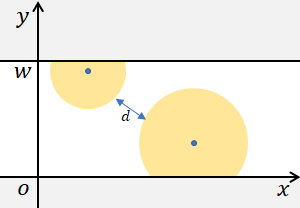
\includegraphics{Official/3.png}
    \end{center}

    为了能够在不触动报警装置的情况下悄悄通过这条走廊,伊森也许需要一些特殊的紧身装备来控制他的身材。同步协助伊森行动的小组成员班吉在收到伊森求助后,立即通过技术手段将整条走廊建模在二维平面上。如上图,整个走廊可以视为二维平面上由 $y=0$ 与 $y=w$ 两条直线所框定的白色区域,中间有若干的报警传感器位于墙壁上或者走廊中。伊森在模型中可以视为具有一定半径的圆,位于走廊的最左侧 $x=-\infty$,想穿过走廊到达最右侧 $x=+\infty$。班吉需要尽快计算出该圆可以具有的最大半径,以便伊森可以悄悄地通过这条走廊而不触发报警装置,聪明的你快帮帮他!


    \InputFile

    第一行输入一个正整数 $T\ (1\le T\le 100)$,表示数据组数。
    
    接下来 $T$ 组数据,每组数据第一行输入一个正整数 $w\ (1\le w\le 10^5)$,表示这条走廊的宽度,建模后墙壁的边缘分别为直线 $y=0$ 与 $y=w$。

    接下来一行输入一个非负整数 $n\ (0\le n\le 10^3)$,表示报警传感器的数目,编号从 $1$ 到 $n$。

    接下来 $n$ 行,第 $i$ 行输入三个整数 $x_i$、$y_i$ 和 $r_i\ (-10^5\le x_i\le 10^5,\ 0\le y_i\le w,\ 1\le r_i\le 10^5)$ 并由空格间隔开,表示传感器建模后的坐标与感知范围。
    
    \OutputFile
    
    对于每组数据,请输出一个浮点数,表示能够顺利通过这条走廊而不触发报警装置的人的最大半径,注意换行。输出结果要求精确到 $10^{-6}$,若精确答案为 $a$,你的输出结果为 $b$,只要满足 $|a-b|<10^{-6}$,评测法官 Jury 就认为你的输出是正确的。

    
    \Example
    
    \begin{example}
    \exmp{
        3
        10
        2
        0 2 3
        12 7 4
        10
        2
        0 2 3
        8 7 4
        10
        2
        0 2 3
        4 7 4
    }{
        1.500000
        1.216991
        0.000000
    }%
    \end{example}

\end{problem}